\section{Design Study}
\label{sec:materiais}

This study conducts a quantitative experimental research by investigating and comparing the performance, computational cost, and CWV metrics analysis between SSR and CSR for data presentation in web applications. The following subsections describe the development environment, which consists of a web application. Subsequently, the materials and methods used in the experiment are detailed, including performance measurement tools, computational cost metrics, and the different data sizes analyzed.

\subsection{Study Steps}

The study was divided into three steps, which are described as follows.

% This section presents the three main stages of development for this study.

In the \textit{first step}, the data were defined and created in JSON format. The datasets were generated in five different sizes: 498 kB, 2 MB, 7.9 MB, 16.8 MB, and 26 MB. Each dataset was composed by combining 13 different images, resulting in: 370 images (498 kB), 1,500 images (2 MB), 6,000 images (7.9 MB), 12,000 images (16.8 MB), and 19,000 images (26 MB).
These sizes were selected based on the study by~\citet{jsonXmlCaseStudy:2009}, which analyzed the performance of data interchange formats in various scenarios. For the experiment, a data structure was designed to simulate a photo gallery system using JSON (Figure~\ref{fig:jsonStructure}). The choice of this data structure aims to represent a real-world use case where user information is frequently exchanged between systems.

\begin{figure}[h]
\centering
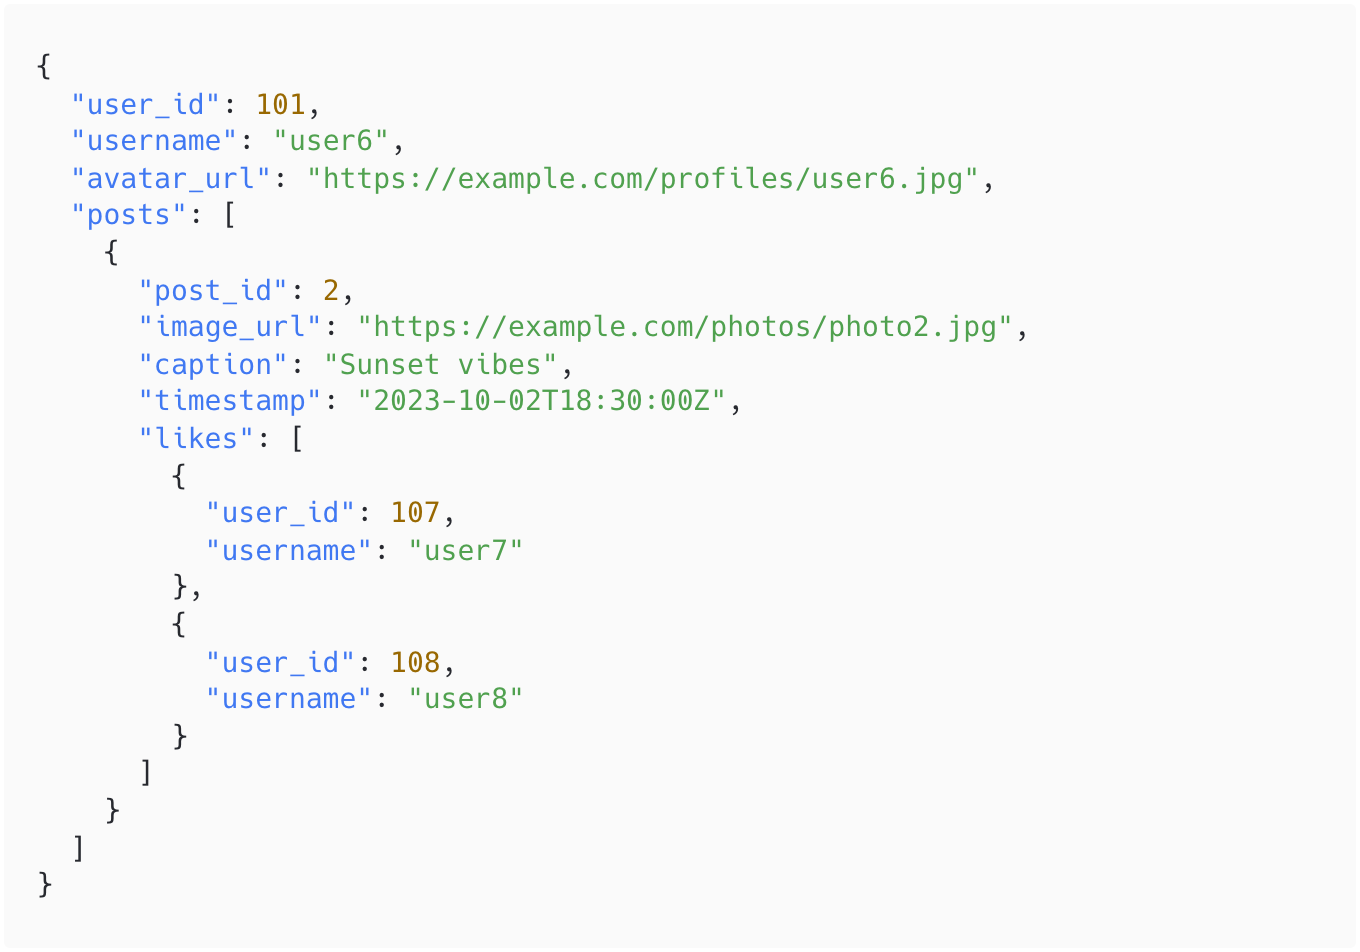
\includegraphics[width=.45\textwidth]{img/03-json-structure.png}
\caption{JSON data structure used in the application}
\label{fig:jsonStructure}
\end{figure}

Furthermore, a back-end application was developed using the NodeJS platform. An Application Programming Interface (API) was created to handle two parameters: data size and rendering type (SSR or CSR). Based on these parameters, the API returns either the HTML rendered from the JSON or the raw JSON itself to the client. The data is stored locally.

The \textit{second step} %involved developing a front-end application in JavaScript. This application (Figure~\ref{fig:exampleFig2}) allows users to select both the size and format of the data to be requested. It then sends the request to the back-end and displays the response, which may either be the fully rendered HTML from the server or the raw JSON used to dynamically build the web page.
consisted of developing a front-end application in JavaScript. As illustrated in Figure~\ref{fig:exampleFig2}, this application enables users to select both the size and format of the data to be requested. Once the request is sent to the back-end, the application displays the response, which can either be the fully rendered HTML returned by the server or the raw JSON used to dynamically build the web page.

\begin{figure}[h]
\centering
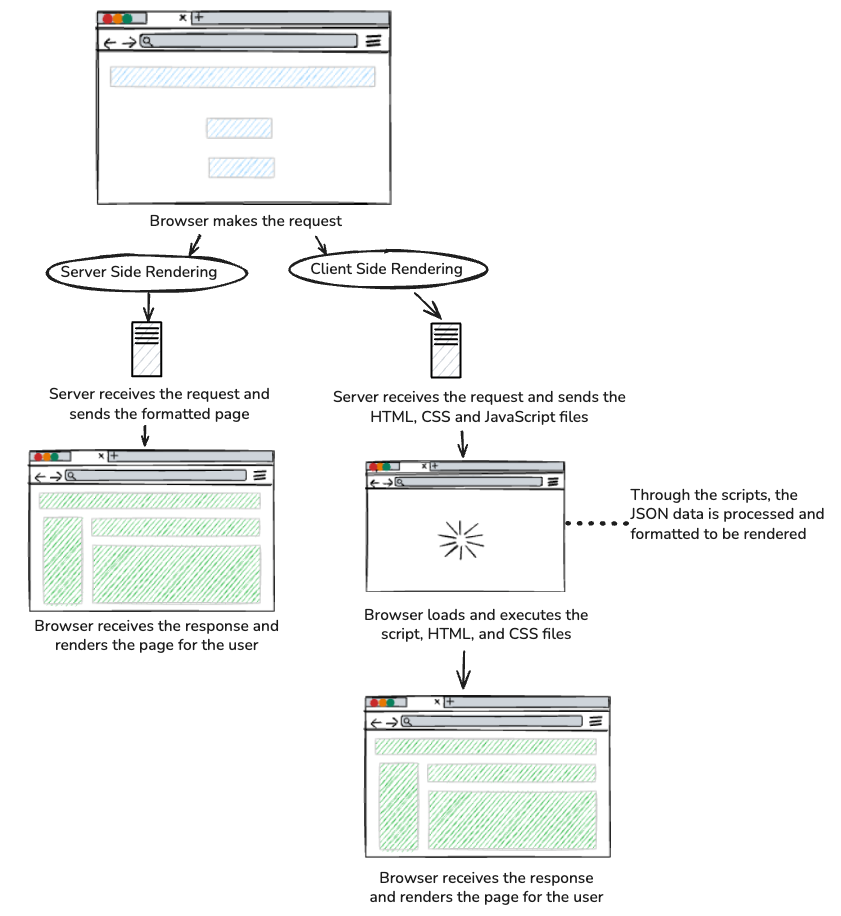
\includegraphics[width=.5\textwidth]{img/04-csr-ssr.png}
\caption{Application operation flow}
\label{fig:exampleFig2}
\end{figure}

Subsequently, a JavaScript script was developed to evaluate application performance. %The script uses the Lighthouse library to automatically calculate key performance metrics. Additionally, the \texttt{chrome-launcher} library was employed to launch a clean instance of the Chrome browser for performance testing. The Puppeteer tool\footnote{\url{https://pptr.dev/}} was also used to collect profiling metrics and computational cost data. Each configuration (JSON and HTML) was tested 10 times, and the average execution time was computed to yield more accurate and representative results. The following metrics, were analyzed in this study:
Leveraging the Lighthouse library, the script automatically computes key performance metrics. To ensure consistent testing conditions, the \texttt{chrome-launcher} library was used to start a clean instance of the Chrome browser. In addition, the Puppeteer tool\footnote{\url{https://pptr.dev/}} was used to collect profiling data and computational cost metrics. Each configuration (JSON and HTML) was tested 10 times, with the average execution time calculated to provide more accurate and representative results. The following metrics were analyzed in this study:

%%=============================
% Pra deixar o texto auto-contido, eu add uma breve explicação. Caso tenha algo errado, favor verificar Joey
% Na real percebi que ja tem explicação delas, exceto a última.
\begin{enumerate}
    \item \textbf{First Contentful Paint}%: Measures the time until the first piece of content (e.g. text or image) renders on the screen.
    \item \textbf{Speed Index}%: Measures how quickly the content within the visible area (viewport) is visually populated.
    \item \textbf{Time to Interactive}%: Measures the time for a page to become fully responsive to user interactions.
    \item \textbf{Largest Contentful Paint}%: Measures the render time of the largest content element (image or text block) within the visible area.
    \item \textbf{\textit{JS Heap} Size}%: Measures memory usage by JavaScript, indicating the application's computational cost.
\end{enumerate}

In the \textit{third step}, the Kruskal-Wallis statistical test\footnote{Kruskal-Wallis is a non-parametric test used for comparing three or more independent samples.} was applied to validate the significance of the results across the different data formats tested. Core Web Vitals metrics were evaluated to understand the impact of data formats on user experience.



\subsection{Development Environment}

All experiments were conducted in a controlled environment to ensure consistency and reproducibility of results. The system's development and execution were performed on a MacBook Air M2, featuring an 8-core \textit{3.5 GHz} CPU, running macOS Sequoia 15.0, equipped with 16GB of RAM and a 256GB SSD.
